% threepennygui-Ht.tex
\begin{hcarentry}[updated]{threepenny-gui}
\label{threepenny-gui}
\report{Heinrich Apfelmus}%05/15
\status{active development}
\makeheader

Threepenny-gui is a framework for writing graphical user interfaces (GUI) that uses the web browser as a display. Features include:

\begin{compactitem}
\item \emph{Easy installation.} Everyone has a reasonably modern web browser installed. Just install the library from Hackage and you are ready to go. The library is cross-platform.
\item \emph{HTML} + \emph{JavaScript}. You have all capabilities of HTML at your disposal when creating user interfaces. This is a blessing, but it can also be a curse, so the library includes a few layout combinators to quickly create user interfaces without the need to deal with the mess that is CSS. A foreign function interface (FFI) allows you to execute JavaScript code in the browser.
\item \emph{Functional Reactive Programming (FRP)} promises to eliminate the spaghetti code that you usually get when using the traditional imperative style for programming user interactions. Threepenny has an FRP library built-in, but its use is completely optional. Employ FRP when it is convenient and fall back to the traditional style when you hit an impasse.
\end{compactitem}

\subsubsection*{Status}

The project is alive and kicking, the latest release is version \verb`0.6.0.1`. You can download the library from Hackage and use it right away to write that cheap GUI you need for your project. Here a screenshot from the example code:

%**<img width=700 src="./chat.jpg">
%*ignore
\begin{center}
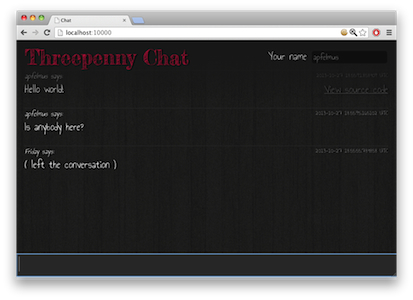
\includegraphics[width=0.5\textwidth]{html/chat.jpg}
\end{center}
%*endignore

For a collection of real world applications that use the library, have a look at the gallery on the homepage.

Compared to the previous report, the communication with the web browser has been overhauled completely. Internally, Threepenny implements a HTTP server that sends JavaScript code to the web browser and receives JSON data back. However, to the library user, this is presented as a \emph{JavaScript foreign function interface}. The module \verb`Foreign.JavaScript` gives you the essential tools needed to manipulate JavaScript objects, call functions, and even export Haskell functions to be called from JavaScript. Moreover, the FFI also handles garbage collection. The GUI parts of the library are built on top of this FFI, but you can also use it independently if you like.

\subsubsection*{Current development}

The library is still very much in flux, significant API changes are likely in future versions. The goal is to make GUI programming as simple as possible, and that just needs some experimentation.

In future versions of Threepenny, I hope to focus on making the process of designing of a GUI simpler and faster. Unfortunately, creating a GUI with HTML and CSS usually takes a significant amount of design work. My hope is that this work can be reduced by offering a default style, incorporating an existing HTML UI kit, and packaging everything in a nice set of combinators.

\FurtherReading
\begin{compactitem}
\item Project homepage: \url{http://wiki.haskell.org/Threepenny-gui}
\item Example code: \url{https://github.com/HeinrichApfelmus/threepenny-gui#examples}
\item Application gallery: \url{http://wiki.haskell.org/Threepenny-gui#Gallery}
\end{compactitem}
\end{hcarentry}
